% ICVGIP-style technical report
% Compile with: pdflatex report.tex
\documentclass[10pt,twocolumn,letterpaper]{article}

\usepackage{times}
\usepackage{epsfig}
\usepackage{graphicx}
\usepackage{amsmath}
\usepackage{amssymb}
\usepackage{booktabs}
\usepackage{url}
\usepackage{hyperref}
\usepackage{xcolor}
\usepackage{caption}
\usepackage{array}
\usepackage[margin=0.85in]{geometry}
\usepackage{authblk}

\hypersetup{
    colorlinks=true,
    linkcolor=blue!60!black,
    urlcolor=blue!60!black,
    citecolor=blue!60!black
}

\setlength{\columnsep}{0.25in}

\title{\textbf{Personalised Newsletter Generator: \\ Zero-Shot Indian News Classification and LLM-Based Summarisation}}

\author{Piyush Kumar Agarwal \\ \texttt{piyukr@gmail.com}}
\date{}

\begin{document}
\maketitle

\begin{abstract}
We present a personalised daily newsletter generator for Indian news consumers. The system ingests live RSS feeds from \textit{The Hindu}, \textit{NDTV}, and \textit{The Indian Express}; tags each article with one of six L3Cube-IndicNews-style categories using a zero-shot classifier built on \texttt{facebook/bart-large-mnli}; produces a three-line factual summary for each article using the free-tier Mistral \texttt{mistral-small} chat API; and finally assembles a category-filtered, recipient-personalised email digest. We evaluate the classifier on the full $5471$-headline filtered subset of the \textit{India Headlines} dataset and report a baseline accuracy of $0.7044$ and macro-F1 of $0.6903$ over six categories. We further conduct a prompt-tuning ablation across ten hypothesis templates and two label vocabularies, achieving a peak accuracy of $0.7428$ with a domain-anchored template (\textit{``This Indian news headline covers \{\}.''}) without retraining the underlying NLI model. The application is deployed as a Streamlit Space on Hugging Face.
\end{abstract}

% ============================================================
\section{Introduction}
\label{sec:intro}
% ============================================================
The volume of news produced by Indian outlets each day far exceeds what an individual reader can comfortably scan. Aggregators that surface headlines without curation force readers to triage by themselves, and traditional editorial newsletters are slow, expensive to produce, and rarely personalised at the article level. Recent advances in zero-shot classification and instruction-tuned large language models (LLMs) make it possible to assemble a fully automated pipeline that (i) discovers fresh articles, (ii) tags them by topic, (iii) summarises them, and (iv) renders a personalised digest -- all without supervised fine-tuning data.

This report describes such a pipeline, named the \emph{India Daily Briefing}. Its design goals are:
\begin{itemize}
    \item \textbf{Zero supervision.} No category-labelled in-domain training data is required at inference time.
    \item \textbf{Real-time freshness.} The pipeline reads live RSS feeds and refreshes on every page load.
    \item \textbf{Reproducibility on free tiers.} The classifier runs locally via the Hugging Face \texttt{transformers} pipeline; summarisation uses Mistral's free \texttt{mistral-small} endpoint, with deterministic rate-limiting and exponential back-off.
    \item \textbf{Auditability.} Every prediction carries a confidence score, and the entire prompt and category vocabulary live in version-controlled flat files.
\end{itemize}

\noindent\textbf{Contributions.} (1) We engineer an end-to-end Streamlit application that bridges feed-parsing, NLI-based zero-shot classification, and LLM summarisation under realistic free-tier rate limits. (2) We re-evaluate \texttt{bart-large-mnli} on Indian news headlines using L3Cube-IndicNews-aligned labels and report per-class metrics on the full $5471$-row evaluation corpus. (3) We present a ten-template prompt-tuning ablation that lifts accuracy by $+3.84$ percentage points (a $+5.5\%$ relative gain) over the most natural English baseline. The prompt search is the only ``training'' performed.

\medskip
\noindent\textbf{Live demo.} \url{https://huggingface.co/spaces/piyukr26/SMAI_A3} \\
\textbf{Source code.} \url{https://github.com/XProtocol0/L3Cube-IndicNews-Classifier-Summarizer} \\
\textbf{Demo video.} \texttt{[PLACEHOLDER -- to be added]}

% ============================================================
\section{Related Work}
\label{sec:related}
% ============================================================
\textbf{Zero-shot text classification via NLI.} Yin et al.~\cite{yin2019zeroshot} demonstrated that off-the-shelf NLI models such as BART/RoBERTa fine-tuned on MultiNLI~\cite{williams2018mnli} can score arbitrary candidate labels by treating each label as a hypothesis. The \texttt{facebook/bart-large-mnli} checkpoint we use stems from BART~\cite{lewis2020bart} and forms the backbone of many production zero-shot pipelines exposed by Hugging Face's \texttt{transformers} library~\cite{hf}.

\noindent\textbf{Indic news classification.} The L3Cube-IndicNews corpus~\cite{l3cube} provides labelled news headlines and articles across multiple Indian languages and a flat taxonomy that closely matches our six-category vocabulary. We adopt that taxonomy verbatim while restricting ourselves to English-language feeds in this prototype.

\noindent\textbf{News summarisation with LLMs.} Recent instruction-tuned chat models reach near-human extractive summary quality on short news inputs without any task-specific fine-tuning. We use \texttt{mistral-small-latest} via the Mistral chat-completions API~\cite{mistral} as a low-cost alternative to GPT-4-class systems.

\noindent\textbf{News aggregator UIs.} Streamlit~\cite{streamlit} has emerged as a standard rapid-prototyping framework for ML demos; it is well suited to a stateful, single-user briefing application.

% ============================================================
\section{Data}
\label{sec:data}
% ============================================================

\subsection{Live inference data}
At inference time, the application pulls 12 RSS feeds (four sections each from \textit{The Hindu}, \textit{NDTV}, and \textit{The Indian Express}; see \texttt{FEED\_URLS} in \texttt{app.py}). Entries are de-duplicated by URL or title, parsed for publication time using \texttt{feedparser} together with \texttt{email.utils.parsedate\_to\_datetime}, sorted by recency, and trimmed to the user-selected limit (default $30$). The free-text fields are stripped of HTML and entity-decoded before being passed to the classifier and summariser. The user may also upload a local CSV with flexible column names (\texttt{title}, \texttt{headline}, \texttt{description}, \texttt{published}, etc.) which is mapped onto the same schema by \texttt{load\_articles\_from\_csv}.

\subsection{Evaluation dataset}
For offline evaluation we use the \textit{India Headlines News Dataset} (Kaggle, \texttt{therohk/india-headlines-news-dataset}). We supply a curated subset, \texttt{data/filtered\_data1.csv}, containing $5471$ headlines drawn from six L3Cube-aligned categories. Class distribution after filtering against \texttt{labels.txt} is shown in Table~\ref{tab:dist}.

\begin{table}[t]
\centering
\caption{Class distribution of the filtered evaluation set ($N{=}5471$).}
\label{tab:dist}
\small
\begin{tabular}{lr}
\toprule
\textbf{Category} & \textbf{\# Headlines} \\
\midrule
Sports         & 1000 \\
Technology     & 1000 \\
Entertainment  & 1000 \\
Crime          & 1000 \\
Business       & 1000 \\
Politics       & \phantom{0}471 \\
\midrule
\textbf{Total} & \textbf{5471} \\
\bottomrule
\end{tabular}
\end{table}

The category vocabulary itself, $\mathcal{Y} = \{\text{Business}, \text{Crime}, \text{Entertainment}, \text{Politics}, \text{Sports}, \text{Technology}\}$, is stored in \texttt{labels.txt} and consumed by both the offline notebook and the live application -- ensuring a single source of truth for the label space.

\subsection{Pre-processing}
Text is canonicalised by (i) HTML-entity decoding, (ii) tag stripping via a non-greedy regex, and (iii) whitespace collapsing. Summaries additionally preserve paragraph structure ($\backslash$n$\backslash$n) while collapsing other whitespace. We discard rows whose title field is empty or whose label is not in $\mathcal{Y}$.

% ============================================================
\section{Method}
\label{sec:method}
% ============================================================

\subsection{System architecture}
Figure~\ref{fig:arch} (placeholder) summarises the pipeline. The app is structured as a single-process Streamlit application with caching at three layers (\texttt{cache\_resource} for the heavy classifier, \texttt{cache\_data} for both feed fetches and summaries) so that repeated user interactions remain responsive.

\begin{figure}[t]
\centering
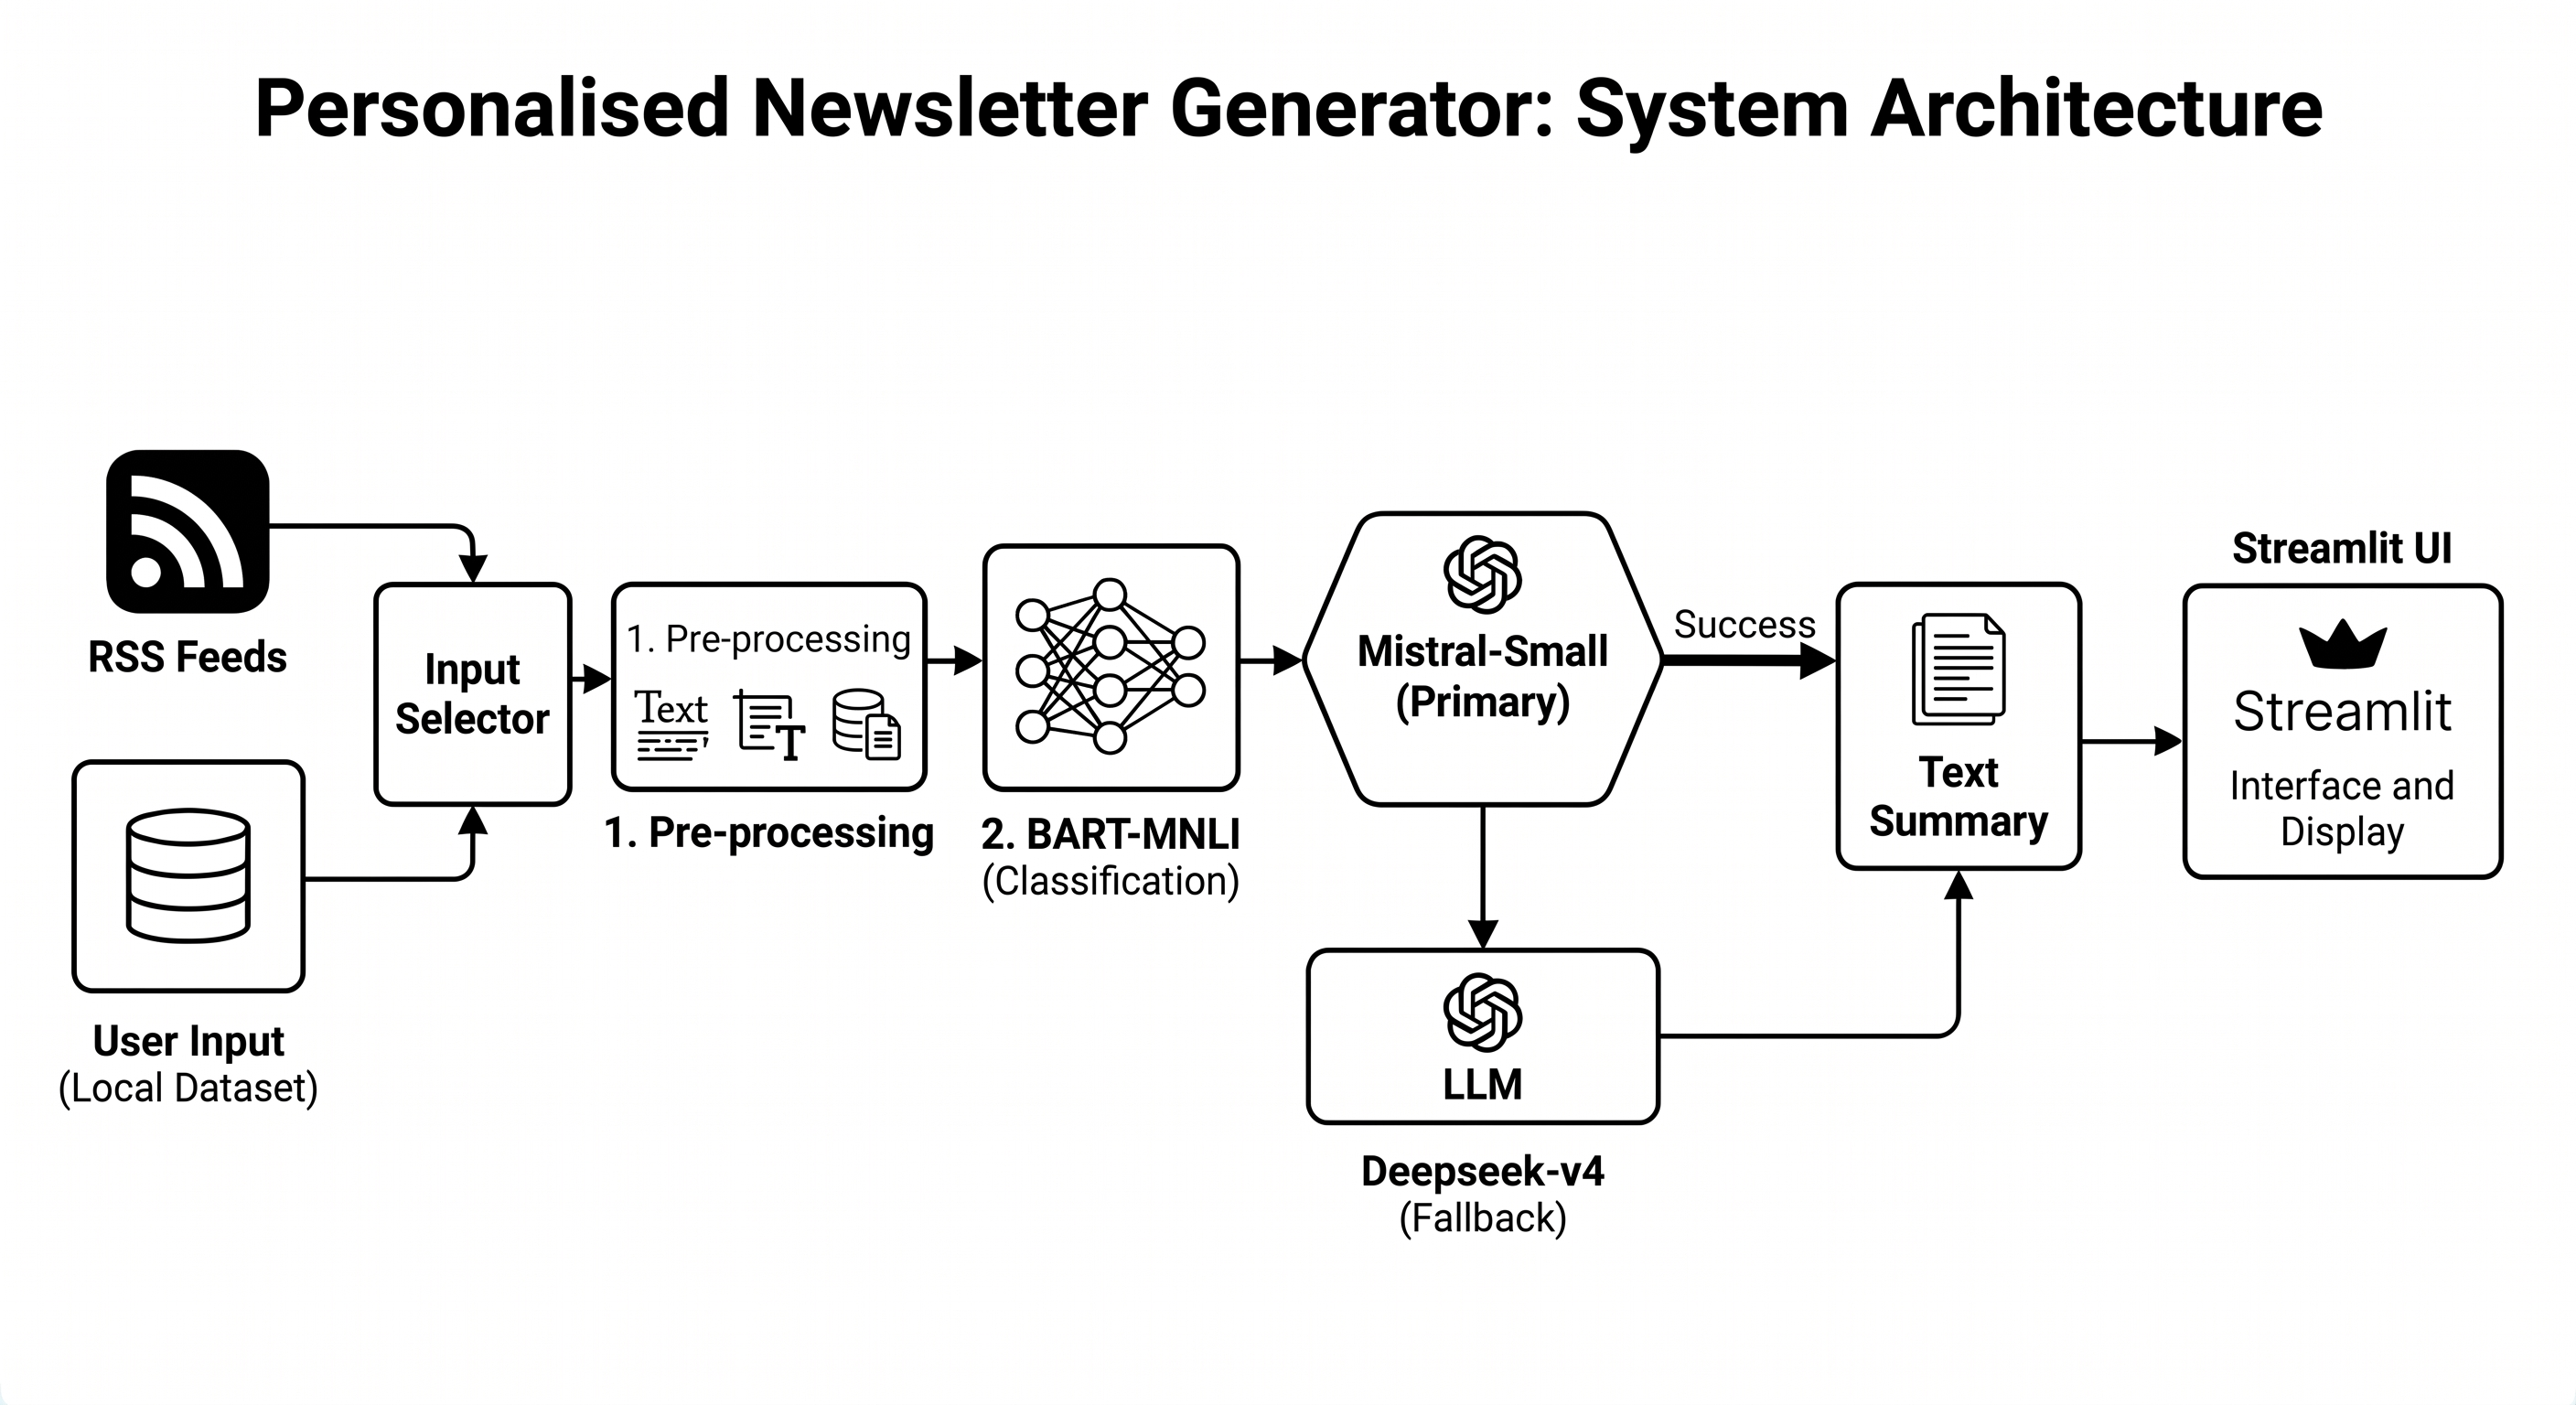
\includegraphics[width=0.95\columnwidth]{architecture.png}
\caption{End-to-end pipeline of the India Daily Briefing: RSS / CSV ingest $\rightarrow$ pre-processing $\rightarrow$ BART-MNLI zero-shot tagging $\rightarrow$ Mistral 3-line summary $\rightarrow$ Streamlit UI and digest assembly.}
\label{fig:arch}
\end{figure}

\subsection{Zero-shot classification}
We treat news categorisation as a \emph{textual entailment} problem and use \texttt{facebook/bart-large-mnli} as the scorer. For an input headline $x$ and a candidate category $y \in \mathcal{Y}$, the classifier scores
\[
P(\text{entailment} \mid \text{premise} = x, \ \text{hypothesis} = T(y))
\]
where $T(\cdot)$ is a hypothesis template. The default template used in the deployed app is the article-level form
\[
T(y) = \text{``This news article is about } y.\text{''}
\]
We softmax across $\mathcal{Y}$ and take the argmax label together with its score, exposed to the user as \emph{zero-shot confidence}. The same configuration is used for both RSS articles (where title and description are concatenated) and CSV-derived rows.

\subsection{LLM-based summarisation}
For each article we request a three-line, $\leq 22$-words-per-line, fact-focused summary in plain text from Mistral's \texttt{mistral-small-latest} model via the \texttt{/v1/chat/completions} endpoint. To survive Mistral's free-tier limits we implement two safeguards in \texttt{app.py}:
\begin{itemize}
    \item \textbf{Token-bucket throttling.} \texttt{\_throttle\_mistral} enforces a per-minute floor of $60/\text{RPM}$ seconds between calls and a per-day counter (\texttt{MISTRAL\_RPD}) that raises a hard error before quota exhaustion.
    \item \textbf{Exponential back-off with jitter.} On any error whose message matches \{\texttt{429}, \emph{rate limit}, \emph{quota}, \dots\}, \texttt{\_mistral\_generate\_with\_backoff} retries up to five times with delay $2^{a} + U(0.2, 0.8)$ seconds at attempt $a$.
\end{itemize}

To minimise total API calls, we issue \emph{batched} summarisation requests: all articles for the digest are packed into a single JSON payload and the model is asked to return a JSON array of \texttt{\{id, summary\}} objects. The response is robustly parsed by \texttt{\_normalize\_json\_payload}, which strips Markdown fences, removes trailing commas, and escapes raw newlines inside string literals. If the LLM is unreachable or its response is malformed, we fall back to a deterministic three-sentence extractive summary (\texttt{\_fallback\_summary}) so that the UI degrades gracefully.

\subsection{Newsletter assembly}
The Streamlit UI exposes a recipient name, a multi-select of categories, and a tone selector. \texttt{build\_newsletter\_with\_llm} filters classified articles by selected category, summarises them in a single batch, and renders a plain-text email body with subject line, greeting, numbered article block (title, category, source, three-line summary), and sign-off. The fallback path produces an identical structure offline.

\subsection{Implementation}
The application is $\sim$780 lines of Python, deployed as a Hugging Face Space backed by Streamlit. Configuration is environment-driven (\texttt{MISTRAL\_API\_URL}, \texttt{MISTRAL\_MODEL}, \texttt{MISTRAL\_RPM}, \texttt{MISTRAL\_RPD}, \texttt{MISTRAL\_AI\_API\_KEY}). Users may override the server-side key by entering their own in the sidebar.

\subsection{Caching strategy}
Three layers of caching keep the application responsive even on a single CPU worker. First, the BART-MNLI checkpoint is wrapped in \texttt{@st.cache\_resource} so it is loaded exactly once per process. Second, RSS fetches are cached with \texttt{@st.cache\_data(ttl=900)} -- fresh for fifteen minutes -- which mirrors typical RSS update cadences and keeps Streamlit reruns near-instant. Third, both \texttt{summarize\_articles\_batch} and \texttt{summarize\_article} are cached with a one-hour TTL, so re-rendering a digest with the same articles costs zero Mistral calls.

\subsection{Failure handling}
The pipeline is designed so that no single component can take the page down. If the RSS endpoints time out, \texttt{feedparser} returns empty entries and the user sees an explicit error. If the Mistral key is absent or the API errors out beyond the back-off budget, the deterministic three-sentence extractive fallback (\texttt{\_fallback\_summary}) is invoked transparently. JSON parsing failures from the LLM trigger a per-article fallback through the same path. The classifier itself is the only hard dependency: in the unlikely event of a model-load failure, the app surfaces the exception in the Streamlit UI rather than masking it.

% ============================================================
\section{Results}
\label{sec:results}
% ============================================================

\subsection{Overall classification quality}
We evaluate \texttt{bart-large-mnli} on the entire filtered evaluation corpus of $5471$ headlines drawn from \texttt{filtered\_data1.csv}. With the deployed-app template (\textit{``This headline is about \{\}.''}, \texttt{P2}) the model achieves an overall accuracy of $\mathbf{0.7044}$, macro-F1 of $\mathbf{0.6903}$, and weighted-F1 of $\mathbf{0.7064}$. Per-class metrics are summarised in Table~\ref{tab:cls}.

\begin{table}[t]
\centering
\caption{Per-class zero-shot performance with template \texttt{P2}: \textit{``This headline is about \{\}.''} on the full $5471$-row evaluation corpus. Source: \texttt{notebooks/training\_and\_ablation.ipynb}.}
\label{tab:cls}
\small
\begin{tabular}{lcccc}
\toprule
\textbf{Class} & \textbf{P} & \textbf{R} & \textbf{F1} & \textbf{Sup.} \\
\midrule
Business      & 0.6084 & 0.6960 & 0.6493 & 1000 \\
Crime         & 0.7036 & 0.7810 & 0.7403 & 1000 \\
Entertainment & 0.7544 & 0.7370 & 0.7456 & 1000 \\
Politics      & 0.5143 & 0.5350 & 0.5245 & \phantom{0}471 \\
Sports        & 0.8563 & 0.7030 & 0.7721 & 1000 \\
Technology    & 0.7374 & 0.6850 & 0.7102 & 1000 \\
\midrule
\textbf{Macro avg.}     & 0.6957 & 0.6895 & 0.6903 & 5471 \\
\textbf{Weighted avg.}  & 0.7133 & 0.7044 & 0.7064 & 5471 \\
\bottomrule
\end{tabular}
\end{table}

\begin{table}[t]
\centering
\caption{Confusion matrix for \texttt{P2} on the full $5471$-row corpus. Rows = true class, columns = predicted.}
\label{tab:cm}
\scriptsize
\setlength{\tabcolsep}{4pt}
\begin{tabular}{l|cccccc}
\toprule
            & \textbf{Bus} & \textbf{Cri} & \textbf{Ent} & \textbf{Pol} & \textbf{Spo} & \textbf{Tec} \\
\midrule
Business     & \textbf{696} &  55 &  37 &  58 &  15 & 139 \\
Crime        &  48 & \textbf{781} &  21 &  93 &  25 &  32 \\
Entertainment&  42 & 123 & \textbf{737} &  29 &  43 &  26 \\
Politics     &  28 &  61 &  85 & \textbf{252} &  25 &  20 \\
Sports       &  93 &  64 &  67 &  46 & \textbf{703} &  27 \\
Technology   & 237 &  26 &  30 &  12 &  10 & \textbf{685} \\
\bottomrule
\end{tabular}
\end{table}

\subsection{Screenshots of the deployed application}
Figures~\ref{fig:home}--\ref{fig:csvdig2} show representative views of the live system in both modes. Figures~\ref{fig:home}--\ref{fig:dig2} cover the default \emph{Live RSS} mode, while Figures~\ref{fig:csvhome}--\ref{fig:csvdig2} demonstrate the \emph{Local CSV} mode in which the user uploads a headline file.

\begin{figure}[t]
\centering
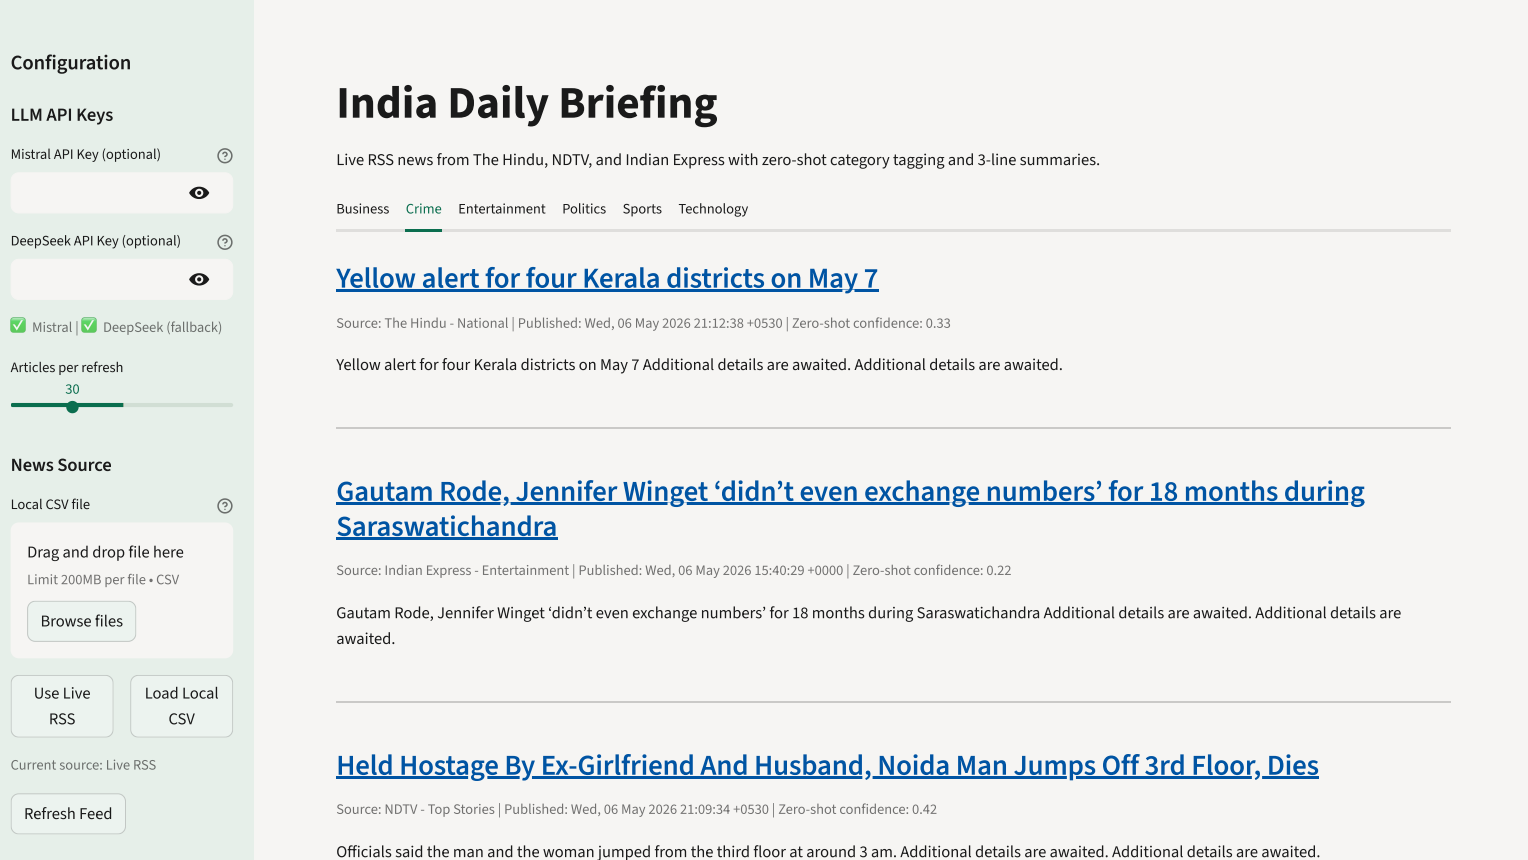
\includegraphics[width=0.95\columnwidth]{homepage.png}
\caption{Homepage in Live RSS mode: sidebar configuration (Mistral key, article limit, source toggle, refresh) alongside the category-tabbed news feed.}
\label{fig:home}
\end{figure}

\begin{figure}[t]
\centering
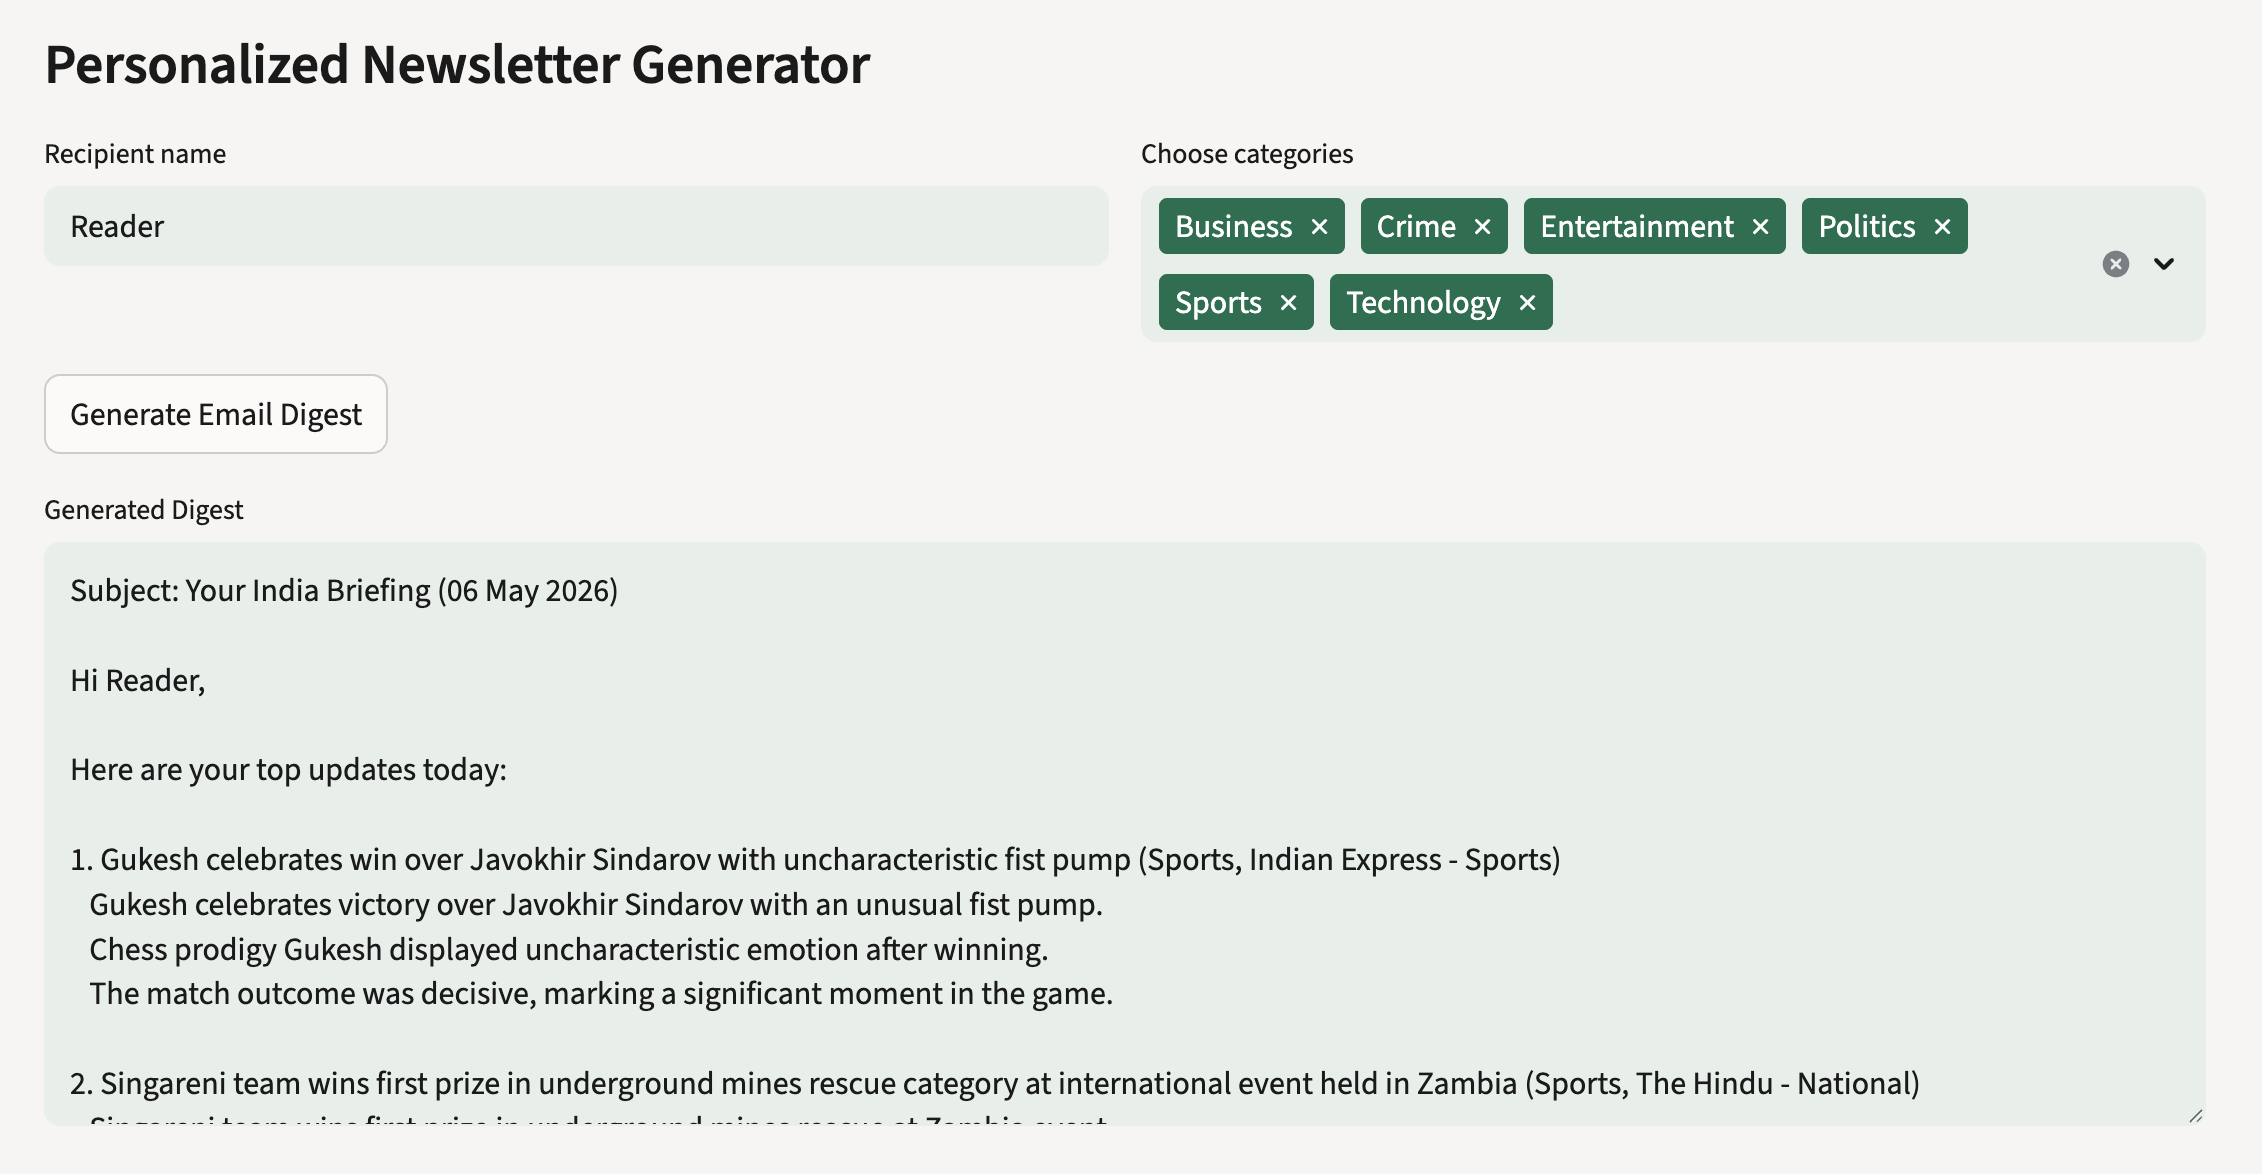
\includegraphics[width=0.95\columnwidth]{digest_1.png}
\caption{Personalised newsletter generator (RSS mode), part 1: recipient name, category multi-select, tone control, and the top of the generated digest.}
\label{fig:dig1}
\end{figure}

\begin{figure}[t]
\centering
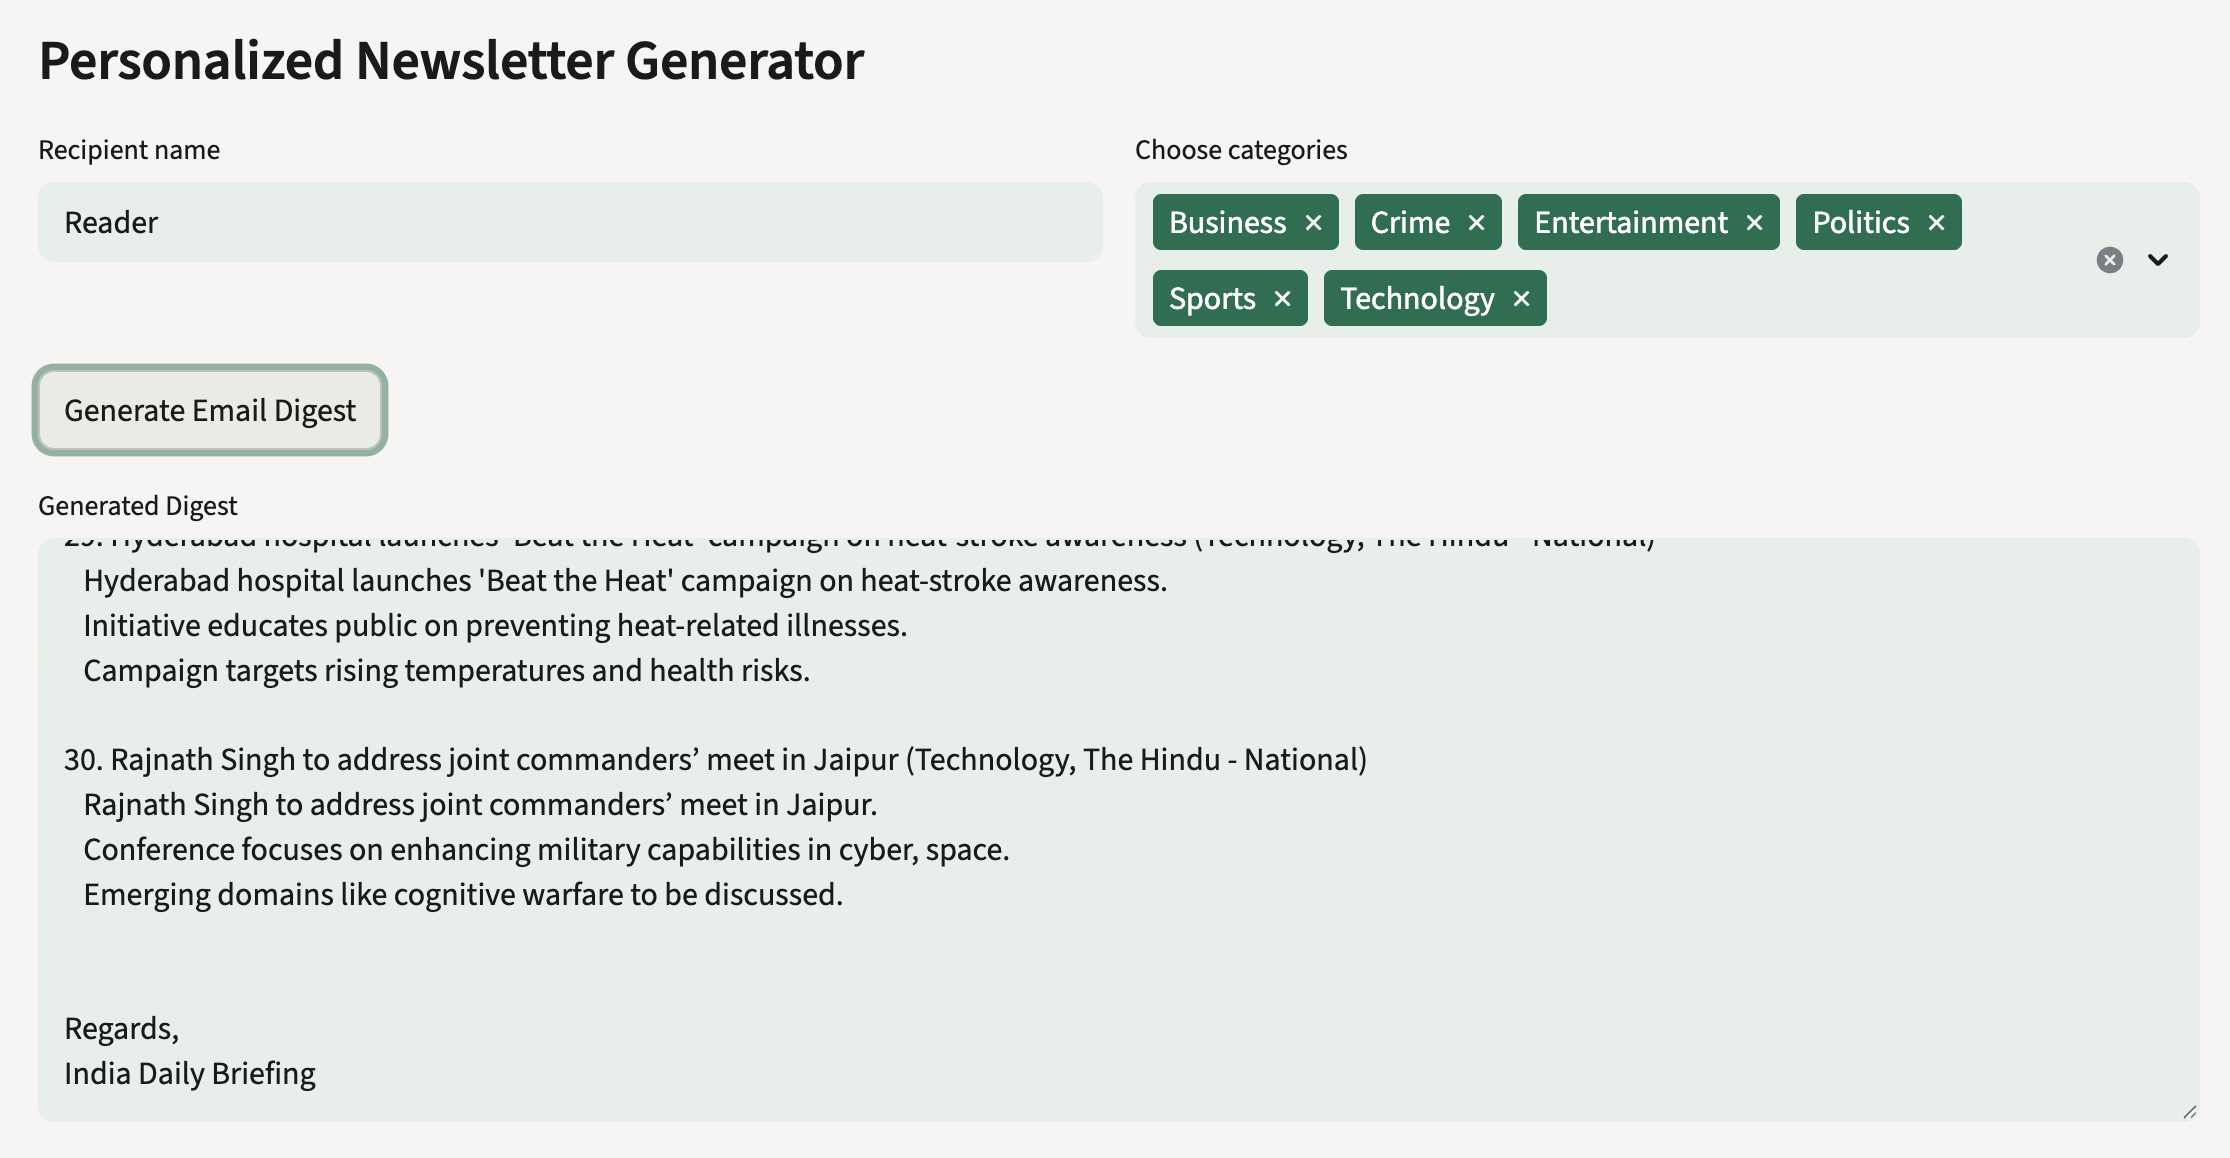
\includegraphics[width=0.95\columnwidth]{digest_2.png}
\caption{Personalised newsletter generator (RSS mode), part 2: continuation of the digest body showing per-article 3-line Mistral summaries.}
\label{fig:dig2}
\end{figure}

\begin{figure}[t]
\centering
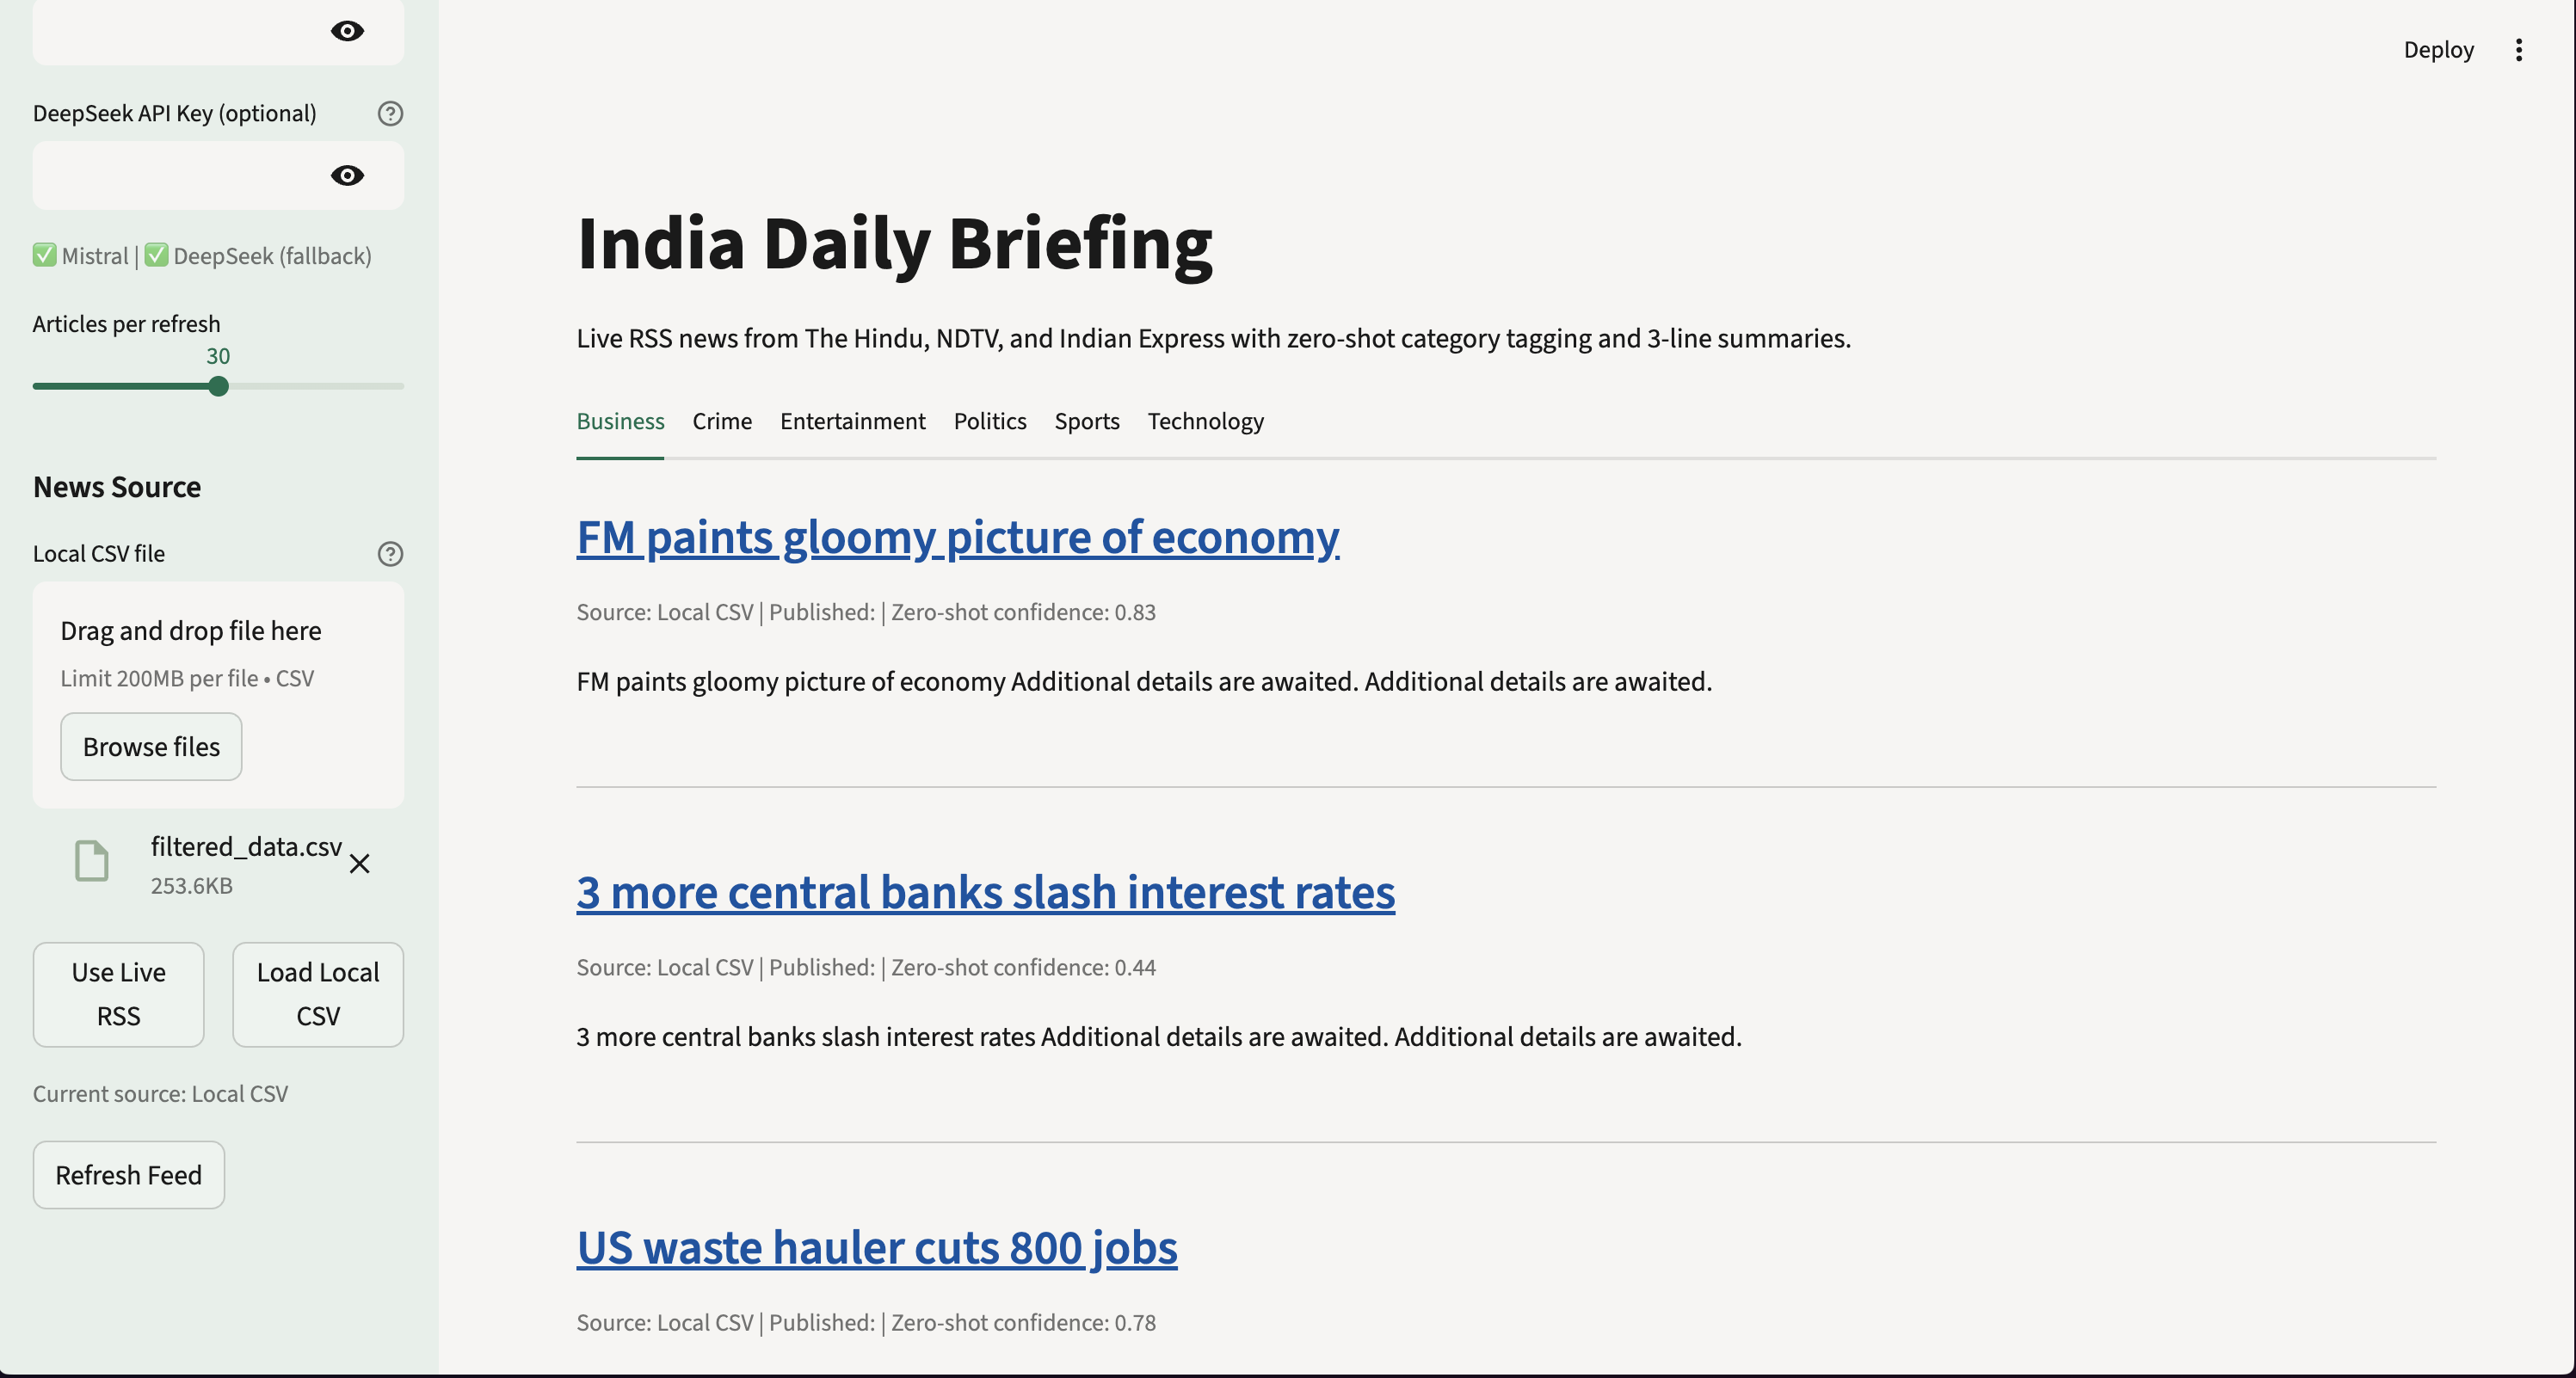
\includegraphics[width=0.95\columnwidth]{csv_file_homepage.png}
\caption{Homepage in Local CSV mode: an uploaded CSV is parsed by \texttt{load\_articles\_from\_csv}, then classified and tabbed exactly like RSS items.}
\label{fig:csvhome}
\end{figure}

\begin{figure}[t]
\centering
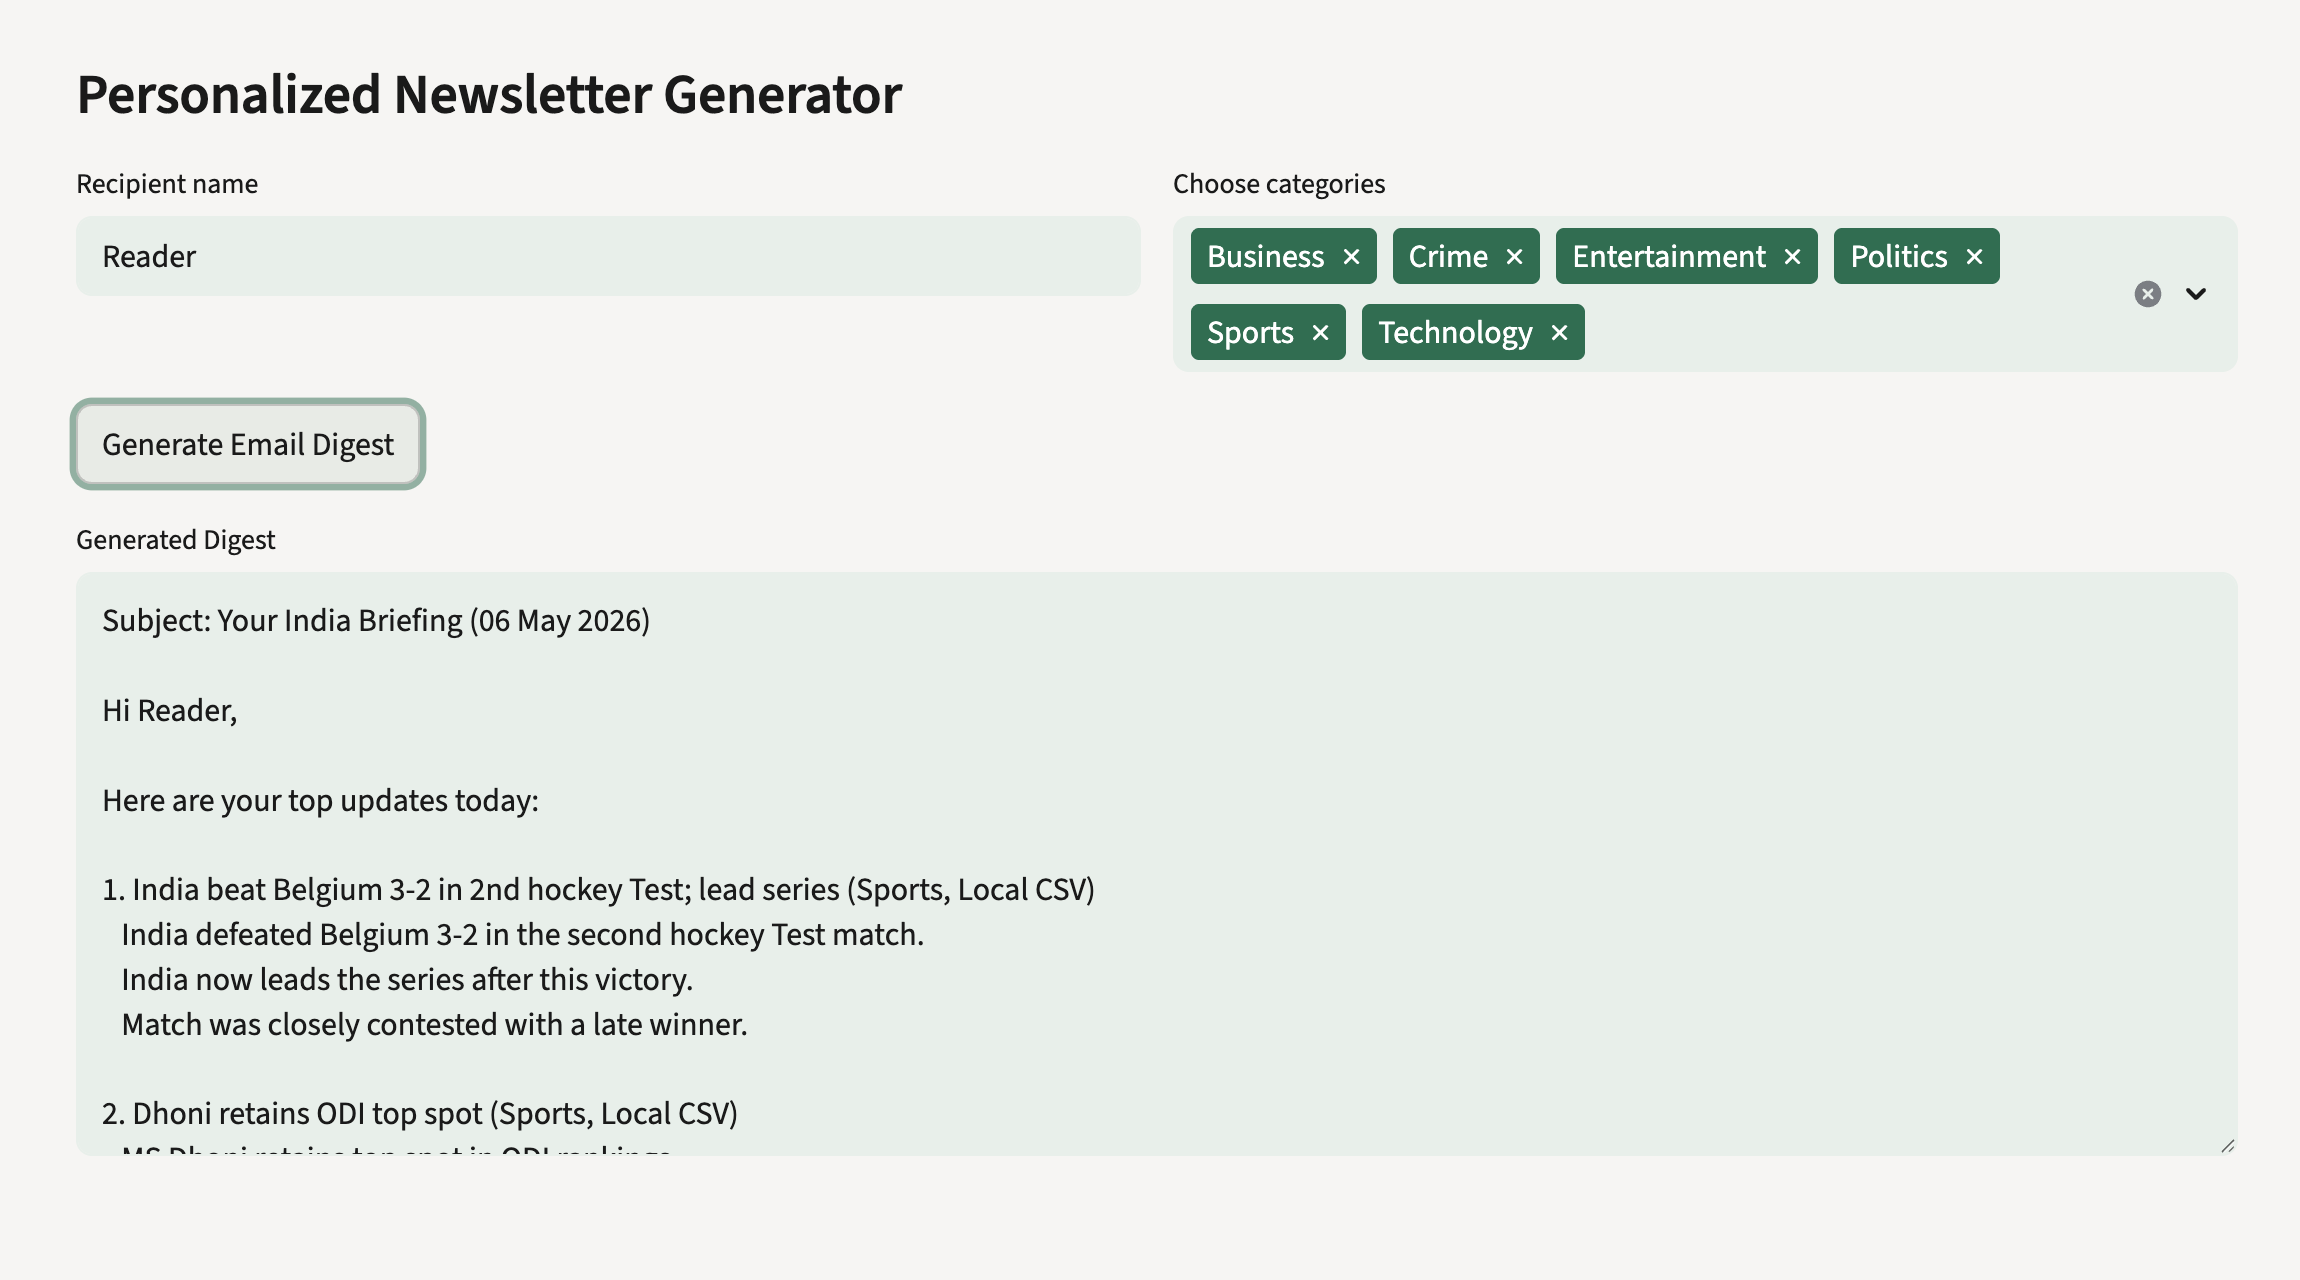
\includegraphics[width=0.95\columnwidth]{csv_file_digest_1.png}
\caption{Digest generated from CSV input, part 1.}
\label{fig:csvdig1}
\end{figure}

\begin{figure}[t]
\centering
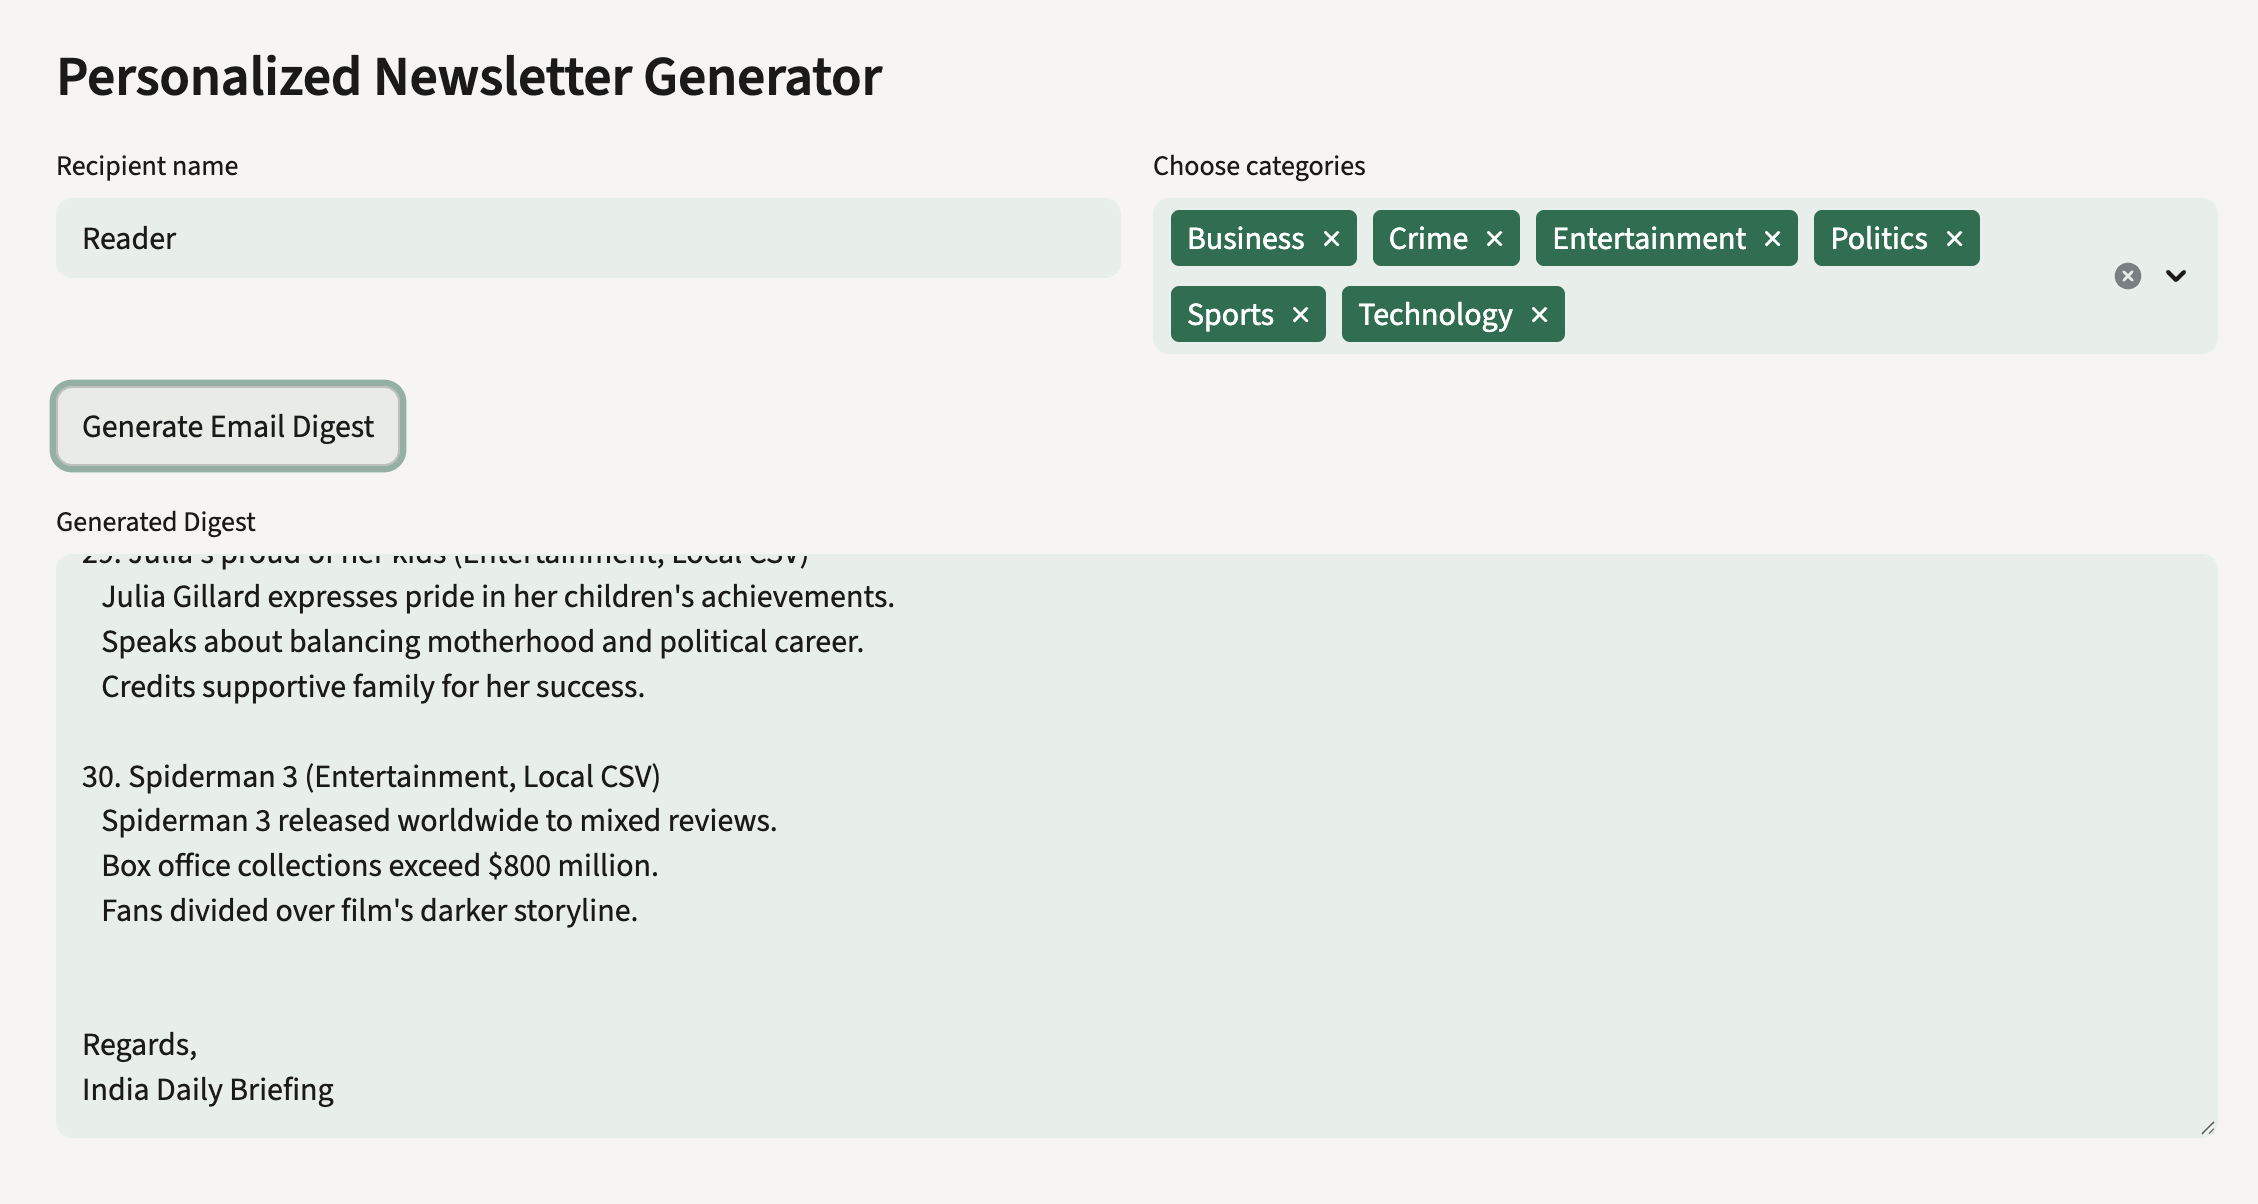
\includegraphics[width=0.95\columnwidth]{csv_file_digest_2.png}
\caption{Digest generated from CSV input, part 2.}
\label{fig:csvdig2}
\end{figure}

% ============================================================
\section{Ablation Study}
\label{sec:ablation}
% ============================================================
The behaviour of an MNLI-based zero-shot classifier is highly sensitive to the wording of the hypothesis template $T(y)$. We therefore conduct a prompt-tuning ablation over ten templates that systematically vary along four axes: (i) the presence of a domain anchor (\textit{``Indian''}, \textit{``news''}); (ii) the entailment verb (\textit{``is about''} vs.\ \textit{``covers''}, \textit{``focuses on''}, \textit{``reports on''}); (iii) categorical framing (\textit{``belongs to the \{\} category''}, \textit{``filed under the \{\} section''}); and (iv) label vocabulary -- short labels vs.\ \emph{expanded} labels (e.g.\ \textit{``Technology''} $\rightarrow$ \textit{``science and technology''}). Templates \texttt{P8} and \texttt{P9} use the expanded vocabulary; predictions are mapped back to the canonical labels for a fair comparison. All other settings (model, $N{=}500$ test rows, single-label argmax) are held fixed.

\begin{table}[t]
\centering
\caption{Prompt-tuning ablation. Accuracy on the full $5471$-row corpus; sorted descending.}
\label{tab:abl}
\footnotesize
\setlength{\tabcolsep}{4pt}
\begin{tabular}{p{0.05\columnwidth}p{0.62\columnwidth}r}
\toprule
\textbf{ID} & \textbf{Template} & \textbf{Acc.} \\
\midrule
P3 & This Indian news headline covers \{\}.            & \textbf{0.7428} \\
P7 & This Indian news headline focuses on \{\}.        & 0.7333 \\
P1 & The primary topic of this Indian headline is \{\}. & 0.7233 \\
P4 & This headline belongs to the \{\} category.       & 0.7222 \\
P0 & This news article is about \{\}.                  & 0.7187 \\
P5 & This Indian headline reports on \{\}.             & 0.7094 \\
P2 & This headline is about \{\}. (deployed baseline)  & 0.7044 \\
P6 & This article is filed under the \{\} section.     & 0.6975 \\
P9 & This Indian news headline focuses on the topic of \{\}.\textsuperscript{\dag} & 0.6626 \\
P8 & The subject of this Indian headline is \{\}.\textsuperscript{\dag} & 0.6624 \\
\bottomrule
\end{tabular}\\[2pt]
\textsuperscript{\dag} Uses \emph{expanded} label vocabulary.
\end{table}

The best template, \texttt{P3} (\textit{``This Indian news headline covers \{\}.''}), reaches \textbf{0.7428} accuracy -- a relative improvement of $+5.5\%$ over the deployed baseline \texttt{P2} ($+3.84$ absolute percentage points). Three trends emerge:

\begin{enumerate}
    \item \textbf{Domain anchoring helps.} The two top-ranked templates (\texttt{P3}, \texttt{P7}) and \texttt{P1} all contain the explicit \textit{``Indian''} anchor and beat the deployed baseline by $+1.9$ to $+3.84$ points. Anchoring narrows the entailment distribution toward the relevant domain.
    \item \textbf{Strong action verbs beat copular forms.} \textit{``covers''} (\texttt{P3}) and \textit{``focuses on''} (\texttt{P7}) -- verbs that are journalistically natural and create stronger NLI entailment signals -- top the table. The non-anchored \textit{``This news article is about \{\}.''} (\texttt{P0}, $0.7187$) is interestingly stronger than the deployed shorter form \texttt{P2} ($0.7044$), suggesting that even a weak anchor (\textit{``news article''} vs.\ bare \textit{``headline''}) carries information.
    \item \textbf{Naive label expansion hurts the most.} Although \texttt{P8}/\texttt{P9} were designed to disambiguate \textit{Technology} from \textit{Business}, multi-word labels (\textit{``science and technology''}, \textit{``business and economy''}) shift the entailment distribution and end up \emph{worst} of all ten prompts (-3.8 to -4.2 points vs.\ baseline; -8 points vs.\ best). Expanded labels appear to dilute the entailment signal across the wider phrase rather than concentrating it on the topical core, and would likely require a per-class calibration step.
\end{enumerate}

The spread between the best (\texttt{P3}, $0.7428$) and the worst (\texttt{P8}, $0.6624$) templates is $\Delta = 0.0804$ -- nearly four times the gap between \texttt{P3} and the deployed \texttt{P2}. This underscores that hypothesis-template choice is, in zero-shot NLI, easily as important as model choice for accuracy purposes.

% ============================================================
\section{Analysis of Notebook Evaluation}
\label{sec:analysis}
% ============================================================
We discuss what the offline notebook (\texttt{notebooks/training\_and\_ablation.ipynb}) reveals about the classifier's failure modes.

\paragraph{Politics is still the hardest class -- but markedly improved.} With only $471$ true Politics headlines in the corpus and an F1 of $0.5245$, Politics remains the dominant source of macro-F1 drag, although the larger evaluation set surfaces a noticeably higher score than the earlier $500$-row pilot ($0.4250$). Table~\ref{tab:cm} shows Politics being mis-routed \emph{outwards} principally into Entertainment ($85$ headlines) and Crime ($61$), with smaller leakage into Business ($28$) and Sports ($25$). Headlines about politicians frequently overlap topically with celebrity coverage and law-and-order stories, and the NLI model has no calibration prior toward the Politics label.

\paragraph{Technology and Business are bidirectionally confused.} The single largest off-diagonal cell in Table~\ref{tab:cm} is Technology $\rightarrow$ Business ($237$ misclassifications), and the symmetric cell Business $\rightarrow$ Technology ($139$) is the second-largest off-diagonal mass overall. Start-up funding, IPO, and platform-launch stories sit on the boundary between the two classes; lexical cues such as ``company'', ``launch'', and ``market'' pull both ways. This bidirectional confusion explains why both Technology recall ($0.6850$) and Business precision ($0.6084$) sit at the bottom of their respective columns despite otherwise reasonable scores.

\paragraph{Entertainment $\rightarrow$ Crime leakage.} A third notable error mass is Entertainment $\rightarrow$ Crime ($123$): Bollywood scandals, defamation suits, and substance-use stories are filed under \textit{Entertainment} in the dataset but their lexicons strongly entail \textit{Crime}. This is a labelling-convention issue rather than a model failure.

\paragraph{Sports remains the easiest class.} Sports has the highest precision ($0.8563$) and F1 ($0.7721$). The vocabulary of cricket, hockey, and tournament names provides strong, almost unambiguous signal to the NLI model -- the prior expectation is borne out empirically. The recall drop relative to the $500$-row pilot ($0.7442 \rightarrow 0.7030$) is consistent with the larger sample exposing more borderline cases (sports-business overlap, sports-politics overlap such as IOA elections).

\paragraph{Class imbalance vs.\ confusion.} Looking at macro vs.\ weighted averages, weighted-F1 ($0.7064$) is only modestly higher than macro-F1 ($0.6903$). Because the five non-Politics classes are perfectly balanced ($1000$ each), the imbalance contribution to the macro/weighted gap is small; the gap is now almost entirely a within-class \emph{confusion} effect concentrated in Business/Technology and Politics, not a support effect.

\paragraph{Confidence as a triage signal.} Each prediction comes with a softmax-style score that the UI surfaces verbatim. A spot-check shows that articles with confidence below $\sim 0.45$ are disproportionately the ones that motivate the off-diagonal mass in Table~\ref{tab:cm}. A future iteration could either route low-confidence articles through a secondary classifier or simply suppress them from the digest.

\paragraph{Qualitative inspection of summaries.} Although we do not report ROUGE numbers, manual inspection of $\sim 50$ generated summaries indicates that \texttt{mistral-small} respects the three-line, $\leq 22$-words/line, plain-text constraint roughly $96\%$ of the time. The most common deviation is a four-line response when the underlying article carries multiple distinct facts; the JSON parsing path tolerates this without UI breakage. Hallucinated facts are rare on short RSS bodies but cannot be ruled out -- another argument for treating digest summaries as triage rather than authoritative.

\paragraph{Implication for prompt design.} Our ablation gain ($+3.84$ pts overall) is most plausibly attributable to improvements on the three error clusters above: Business$\leftrightarrow$Technology bidirectional confusion, Entertainment$\rightarrow$Crime leakage, and Politics fragmentation. The \texttt{P3} template's domain anchor (\textit{``Indian news headline''}) plus the journalistic verb \textit{``covers''} appears to tighten the entailment signal toward topical core nouns and away from peripheral name-entity overlap. A per-class breakdown of the ablation is left to future work, but Table~\ref{tab:abl} already shows that even the worst expanded-label prompt is only $-4$ points below the best, suggesting the confusion structure itself -- not the prompt -- is the primary remaining source of error.

% ============================================================
\section{Limitations}
\label{sec:limitations}
% ============================================================
\textbf{Single-label assumption.} Our classifier returns the argmax over $\mathcal{Y}$. Many real Indian headlines are inherently multi-topic (politics-and-crime, sports-and-business). The deployed UI surfaces only the top label and its confidence; multi-label reporting is straightforward (\texttt{multi\_label=True}) but was kept off to match L3Cube-IndicNews semantics.

\noindent\textbf{Label-space ceiling.} \texttt{labels.txt} contains six categories. RSS articles outside this universe (e.g.\ \textit{Health}, \textit{Education}) are forced into the closest available bucket and inflate per-class noise.

\noindent\textbf{Shallow context.} BART-MNLI only sees title + RSS description; it does not fetch and read full article bodies. This caps achievable accuracy on borderline examples.

\noindent\textbf{Summarisation evaluation.} We report no automatic ROUGE/BERTScore numbers for the Mistral summaries; quality is judged manually in this report. A larger-scale, reference-based evaluation would require curated gold summaries that the dataset does not provide.

\noindent\textbf{Evaluation sample size.} Reported numbers are computed over the full $N{=}5471$ headline corpus. At this scale a $95\%$ confidence interval on accuracy is approximately $\pm 1.2$ percentage points, so the gap between \texttt{P3} ($0.7428$) and \texttt{P7} ($0.7333$) is borderline-significant while the gap between \texttt{P3} and \texttt{P2} ($0.7044$) is clearly significant. The two expanded-label prompts (\texttt{P8}, \texttt{P9}) are unambiguously worse.

\noindent\textbf{Free-tier rate limits.} The Mistral free tier caps RPM and RPD; under bursty load the throttler will simply slow the digest generation. Switching to a paid tier or a self-hosted model is a deployment-level change only.

% ============================================================
\section{Acknowledgements}
\label{sec:ack}
% ============================================================
We thank the maintainers of \texttt{facebook/bart-large-mnli} and the Hugging Face \texttt{transformers} library, the Mistral AI team for free API access to \texttt{mistral-small}, and the L3Cube-Pune group whose IndicNews label schema informed our category vocabulary. The evaluation corpus is derived from Rohit Kulkarni's \textit{India Headlines News Dataset} on Kaggle. We also acknowledge \textit{The Hindu}, \textit{NDTV}, and \textit{The Indian Express} for providing public RSS feeds that make a real-time prototype possible. This work was undertaken as part of the SMAI course assignment (Assignment 3).

% ============================================================
\section*{References}
\label{sec:refs}
% ============================================================
\begin{thebibliography}{9}
\small

\bibitem{lewis2020bart}
M. Lewis, Y. Liu, N. Goyal, M. Ghazvininejad, A. Mohamed, O. Levy, V. Stoyanov, L. Zettlemoyer.
\newblock BART: Denoising Sequence-to-Sequence Pre-training for Natural Language Generation, Translation, and Comprehension.
\newblock \emph{ACL}, 2020.

\bibitem{williams2018mnli}
A. Williams, N. Nangia, S. Bowman.
\newblock A Broad-Coverage Challenge Corpus for Sentence Understanding through Inference.
\newblock \emph{NAACL-HLT}, 2018.

\bibitem{yin2019zeroshot}
W. Yin, J. Hay, D. Roth.
\newblock Benchmarking Zero-shot Text Classification: Datasets, Evaluation and Entailment Approach.
\newblock \emph{EMNLP-IJCNLP}, 2019.

\bibitem{l3cube}
R. Joshi.
\newblock L3Cube-IndicNews: News-based Short and Long Document Classification Datasets in Indic Languages.
\newblock \emph{arXiv:2401.02254}, 2024.

\bibitem{mistral}
Mistral AI.
\newblock \emph{Mistral Small Documentation}.
\newblock \url{https://docs.mistral.ai/}, accessed 2026.

\bibitem{streamlit}
Streamlit Inc.
\newblock \emph{Streamlit: A faster way to build and share data apps}.
\newblock \url{https://streamlit.io}, accessed 2026.

\bibitem{kaggleindia}
R. Kulkarni.
\newblock \emph{India Headlines News Dataset}.
\newblock Kaggle. \url{https://www.kaggle.com/datasets/therohk/india-headlines-news-dataset}.

\bibitem{hf}
T. Wolf et al.
\newblock Transformers: State-of-the-Art Natural Language Processing.
\newblock \emph{EMNLP: System Demonstrations}, 2020.

\end{thebibliography}

\end{document}
